\documentclass[12pt]{article}

%Filter Warning messages, otherwise it would stuff like
\usepackage{silence}
%Disable all warnings issued by latex starting with "You have..."
\WarningFilter{latex}{You have requested package}

%Allgemeine Einstellungen

%Abstände
\usepackage[a4paper,left=3cm,right=3cm,top=3cm,bottom=3.5cm,headsep=12pt]{geometry}%Bottom extra 0.5cm für Footer

%Deutsches Sprachpacket
\usepackage[german,ngerman]{babel}

%For synmbols like \degree
\usepackage{gensymb}

%Times New Roman
\usepackage{mathptmx}

%Titelseite einbinden
\usepackage{pdfpages}

%1.5-Zeilenabstand
\usepackage[onehalfspacing]{setspace}

%Stil der Überschriften, siehe ueberschriften.sty
\usepackage[numeric]{styPackages/ueberschriften}

%Stil des Inhaltsverzeichnisses, siehe inhaltsverzeichnis.sty
\usepackage[numeric]{styPackages/inhaltsverzeichnis}

%Abkürzungsverzeichnis, siehe abk_verzeichnis.sty
\usepackage{styPackages/abk_verzeichnis}

%Stil der Fußzeilen, siehe fusszeilen.sty
\usepackage{styPackages/fusszeilen}

%Literaturverzeichnis und Zitate, siehe literatur.sty
\usepackage{styPackages/bibliography}

%Stil für Header und Footer, siehe header_footer.sty
%Wenn nicht erwünscht, müssen auch die Befehle \frontmatter, \mainmatter auskommentiert werden
\usepackage{styPackages/header_footer}

%Stile für Code-Ausschnitte, siehe codes.sty
\usepackage{styPackages/codes}

%Stile für Anhänge, Bilder, ...
\usepackage{styPackages/anhang}

\usepackage{styPackages/html}

%Silbentrennung (manche Worte werden am Zeilenende nicht getrennt, diese müssen dann nachgetragen werden)
\usepackage[T1]{fontenc}
\hyphenation{öf-fent-lich-en}

%DEBUGGING (Zeigt Boxen an)
%\usepackage{showframe}
\setlength{\skip\footins}{12pt}

\usepackage{makecell}
\usepackage{placeins}

%Anführungszeichen
\usepackage{csquotes}
\MakeOuterQuote{"}

%[H]-Placing
\usepackage{float}

\usepackage{verbatimbox}

\addto\captionsngerman{\renewcommand{\figurename}{Abb.}}
\addto\captionsngerman{\renewcommand{\tablename}{Tab.}}

%Tabellen oder Bilder mit Textumfluss
\usepackage{wrapfig}
\usepackage{etoolbox}
\BeforeBeginEnvironment{wraptable}{\setlength{\intextsep}{1pt}}
\usepackage[justification=centering]{caption}

%Helvetica font
\usepackage{helvet}
%\renewcommand{\familydefault}{\sfdefault}

%Bookmarks and querverweise
\newcounter{dummy}
\usepackage[hidelinks,bookmarks=true]{hyperref}
\usepackage{bookmark}

%Linebreaks Bib und URL
\usepackage[copyfonts,activate={true,nocompatibility},final,tracking=true,kerning=true,spacing=true,factor=1000,stretch=10,shrink=10]{microtype}
\SetExpansion
[ context = sloppy,
  stretch = 30,
  shrink = 60,
  step = 5 ]
{ encoding = {OT1,T1,TS1} }
{ }

\urlstyle{same}

\renewcommand\UrlFont\itshape

\usepackage{xurl}

\begin{document}

\renewcommand{\mytitle}{Documentation\\English}%Titel für oben links
\renewcommand{\myauthor}{Max Mustermann}%Name für unten links
\renewcommand{\headheight}{27pt}%Bei Mehrzeiligem Titel muss Headerhöhe angepasst werden

\setPlainPageStyle{\mytitle}{\nouppercase\plaintitle}{\myauthor}{\thepage}

\setMainPageStyle{\mytitle}{\nouppercase\parttitle}{\myauthor}{\thepage}

%\includepdf[pages={1-}]{titelseite.pdf}

\frontmatter%Stil des Headers/Footers ändern

\pagenumbering{Roman}

\addcontentsline{toc}{part}{Abkürzungsverzeichnis}%Abk-Verz. ins Inhaltsverzeichnis
\printabbreviations%abk_verzeichnis.sty
\clearpage
\renewcommand{\plaintitle}{Abbildungsverzeichnis}
\addcontentsline{toc}{part}{Abbildungsverzeichnis}
{\def\makebox[#1][#2]#3{#3}%
    \listoffigures
}
\clearpage
\renewcommand{\plaintitle}{Tabellenverzeichnis}
\addcontentsline{toc}{part}{Tabellenverzeichnis}
{\def\makebox[#1][#2]#3{#3}%
    \listoftables
}
\clearpage
\renewcommand{\plaintitle}{Inhaltsverzeichnis}%Titel für oben Rechts
%Defbox, damit gepunktete Linie bis zur Zahl geht
{\def\makebox[#1][#2]#3{#3}%
    \tableofcontents
}

\addtocontents{toc}{\vspace{24pt}}%Freiraum im ToC

\clearpage
\mainmatter%Stil des Headers/Footers ändern
\pagenumbering{arabic}

\part{Introduction}
Welcome to \textit{ThesorTeX}! This document shows you how to use the template and the tool. Please also have a look at the FAQ on the website.
To understand this template and the tool, some knowledge of \textit{LaTeX} is required. If you don't understand something, just google it and you might find some answers. If you have problems with the template or the tool, feel free to create an issue in \href{https://github.com/TimoSto/ThesorTeX/issues}{Github}.

\part{use of the template}
The template is available for download as a ZIP file at \url{https://thesortex.com/#/downloads}. When you unzip it, you should see the following structure:
\begin{itemize}
\setlength\itemsep{.15em}
\item \textbf{data/...}: These files are only important if you want to use the tool for literature management. Otherwise you can delete or ignore this folder.
\item \textbf{styPackages/...}: This folder contains style files for the template. You could also write the style declarations directly in the \textit{main.tex}, but then it would become too long.
\item \textbf{abkuerzungen.csv}: This is where you list the abbreviations that should be listed in your paper. You can simply add them separated by a semicolon.
\item \textbf{bib{\_}entries.csv}: Your literature entries are listed here in CSV format. This file is also primarily intended for use with the tool. However, you can also use it without.
\item \textbf{citedKeys.csv}: Suppose you have some entries in your bibliography that are never cited. With this list you can keep them out of the bibliography without losing the entry itself.
\item \textbf{main.tex}: This is where most of the music happens! Because this is where you write your text, insert lists, pictures or tables and call up quotations. More on this below.
\end{itemize}

\section{How can I change the numbering of the headings?}
The numbering can be purely numeric or alphanumeric:
\begin{center}
\begin{figure}[!h]
  \centering
  \begin{minipage}[b]{0.4\textwidth}
    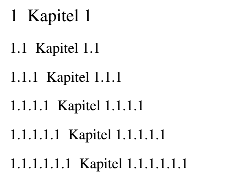
\includegraphics[width=\textwidth]{images/numericChapters.png}
    \caption{Numeric counting}
  \end{minipage}
  \hfill
  \begin{minipage}[b]{0.4\textwidth}
    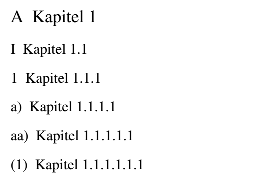
\includegraphics[width=\textwidth]{images/alphaNumericChapters.png}
    \caption{Alphanumeric Counting}
  \end{minipage}
\end{figure}
\end{center}
\noindent The change is made via the parameter in the following packages:
\begin{lstlisting}
\usepackage[numeric]{styPackages/ueberschriften}
\usepackage[numeric]{styPackages/inhaltsverzeichnis}
\end{lstlisting}
resp.
\begin{lstlisting}
\usepackage[alphaNumeric]{styPackages/ueberschriften}
\usepackage[alphaNumeric]{styPackages/inhaltsverzeichnis}
\end{lstlisting}

\section{How can I change the header and footer?}
There is room for a total of four items of information in the header and footer. In the Stadnard configuration these are:
\begin{itemize}
\item Top left: The title of your work
\item Top right: The title of the current upper chapter (\textit{\textbackslash part})
\item Bottom left: Your name
\item Bottom right: The current page number
\end{itemize}
But you can easily change that. The configuration for this example is:
\begin{lstlisting}
\renewcommand{\mytitle}{Documentation\\English}
\renewcommand{\myauthor}{Max Mustermann}
\renewcommand{\headheight}{27pt}

\setPlainPageStyle{\mytitle}{\nouppercase\plaintitle}{\myauthor}{\thepage}

\setMainPageStyle{\mytitle}{\nouppercase\parttitle}{\myauthor}{\thepage}
\end{lstlisting}
You may wonder why there are two different styles. The \textit{MainPageStyle} is meant for the text part. In the top right-hand corner, it contains the title of the current chapter (\textit{\textbackslash part}/\textit{\textbackslash parttitle}). The \textit{PlainPageStyle} contains a value that can be freely chosen by you. This is used for the table of contents, for example.
You can adapt both styles according to your wishes:
\begin{lstlisting}
\setPlainPageStyle{TOP LEFT}{TOP RIGHT}{DOWN LEFT}{DOWN RIGHT}

\setMainPageStyle{TOP LEFT}{TOP RIGHT}{BOTTOM LEFT}{BOTTOM RIGHT}
\end{lstlisting}
Switching between the two styles is done using the commands \textit{\textbf{\textbackslash frontmatter}} and \textit{\textbf{\textbackslash mainmatter}}.

\section{How can I add abbreviations to the list of abbreviations?}
The list of abbreviations is read from the file \textbf{\textit{abbreviations.csv}}. There you can list your abbreviations in the following format:
\begin{quote}
\textit{\textbf{Abk};\textbf{Bed};}\\
\textit{E.G..;Example given;}\\
\textit{...}
\end{quote}

\section{How can I create bibliography entries?}
\begin{quote}
It is recommended to use the Literature Manamement Tool for this purpose. In principle, however, it is also possible without it.
\end{quote}
To answer this question, we have to go a little further. A literature entry has three properties:
\begin{itemize}
\item A unique key
\item A category
\item A list of fields (text values)
\end{itemize}
The entries are read from the file \textit{bibEntries.csv}. For each entry, a literature entry or citation is then created depending on the category.
A category has the following properties:
\begin{itemize}
\item A unique name
\item A list of fields for the bibliography.
\item A list of fields for citations
\end{itemize}
A field in turn has the following properties:
\begin{itemize}
\item A name
\item A prefix and suffix
\item A style (italic or normal)
\end{itemize}
The TeX definition of the entries in the bibliography and the citations can be found in \textit{styPackages/bibliography.sty}. Let's take a look at the category \textit{CitaviArticle} as an example:
\begin{lstlisting}
\newcommand{\printCitaviArticle}[0]{%
    \hangindent=\bibparindent%
    \parindent 0pt%
    \hangafter=1%
    \argI (\argII): \textit{\argIII} In: \textit{\argIV} \argV, \argVI%
    \\%
    \vspace{-12pt}%

}
\end{lstlisting}
This command first ensures that the text is inserted from the second line onwards. Then the fields of the entry are output in the format defined for the category.\\
Citations are defined in principle according to the same scheme:
\begin{lstlisting}
\newcommand{\citeCitaviArticle}[0]{%
    \argVII (\argII), %
}
\end{lstlisting}
Here, the field in position seven is output first, which is not present in the literature entry. This could be, for example, the author's surname, whereas the full name appears in the bibliography. Field 2 is output next. This matches the bibliography. This can be, for example, the year, which has the same value in the bibliography and in citations. However, the format can be different if you want it to be.\\
An entry in \textit{bibEntries.csv} for the category \textit{CitaviArticle} would look like this:
\begin{quote}
testEntry;CitaviArticle;Peter Bunny;1999;ThesorTeX - A great tool;Magazine\_ xy;pP.20-22;https:/doi.org/xyz;Bunny;;;;;;;;;;;;;;;;;;;
\end{quote}
You can see the result in the bibliography. Note that some special characters, e.g. \_ are preallocated by Latex and therefore have to be escaped and replaced by the respective TeX command \\.
You can cite this entry with the command \textit{\textbackslash citebib\{testEntry\}\{cf. \}\{S.10\}}.\citebib{testEntry}{vgl. }{S.10} The second and third arguments are optimal, so they can be left empty (\textit{\textbackslash citebib\{testEntry\}\{\})}.\citebib{testEntry}{ }{ }

\section{How can I add and list attachments?}
Attachments can be output separately numbered. You can use the following commands as headings:
\begin{itemize}
\item \textit{\textbackslash anhang}
\item \textit{\textbackslash anhangI}
\item \textit{\textbackslash anhangII}
\end{itemize}
The list of attachments can be output using the following command:
\begin{lstlisting}
\listofanhang
\end{lstlisting}

\clearpage
\frontmatter%Stil des Headers/Footers ändern
\renewcommand{\plaintitle}{Literaturverzeichnis}
\pagenumbering{Roman}
\setcounter{page}{5}
\addtocontents{toc}{\vspace{24pt}}
\addcontentsline{toc}{part}{Literaturverzeichnis}%Literatur-Verz. ins Inhaltsverzeichnis
\printMyBibliography
\clearpage
\renewcommand{\plaintitle}{Anhang}
\addcontentsline{toc}{part}{Anhang}
{\def\makebox[#1][#2]#3{#3}%
    \listofanhang
}
\clearpage
\anhang{Test Anhang}
Mein erster Anhang

\end{document}